\documentclass{article}
\usepackage[utf8]{inputenc}
\usepackage{amsmath}
\usepackage{amssymb}
\usepackage{graphicx}
\usepackage{bm}
\usepackage{dcolumn}
\usepackage{array}
\usepackage{mathtools}

\newcolumntype{2}{D{.}{}{2.0}}

\graphicspath{{Images/}}


\setlength{\oddsidemargin}{0in}
\setlength{\textwidth}{6.5in}
\setlength{\topmargin}{-.55in}
\setlength{\textheight}{9in}
\pagestyle{empty}

\title{Modern Algebra HW2}
\author{Michael Nameika}
\date{September 2022}

\begin{document}

\maketitle

\Large{\textbf{Section 4 Problems}}

31. If $*$ is a binary operation on a set $S$, an element $x$ of $S$ is an \textbf{idempotent for} $*$ if $x * x = x$. Prove that a group has exactly one idempotent element.
\newline

Proof: Let $\langle G, * \rangle$ be a group. Since $\langle G, * \rangle$ forms a group, we have that there exists a unique identity element $e \in G$ such that for all $a \in G$, $a * e = e * a = a$. It follows then that $e * e = e$. That is, $e$ is an idempotent for $*$. We now wish to show that $e$ is the only idempotent for $*$. Suppose that $e' \in G$ is another idempotent element for $*$. That is, $e' * e' = e'$. Now since $e' \in G$ and $\langle G, * \rangle$ is a group, there exists an inverse $\bar{e} \in G$ of $e'$ such that $e' * \bar{e} = \bar{e} * e' = e$.
Then compose $e' * e' = e'$ on the left with $\bar{e}$:
\[\bar{e} * (e' * e') = \bar{e} * e'\]
by the associative property, the above can be rewritten as
\[(\bar{e} * e') * e' = \bar{e} * e'\]
since $\bar{e} * e' = e$ we have
\[e * e' = e\]
\[e' = e\]
That is, and idempotent element for a group is $e$, the identity element, and is the only idempotent element.
\newline\newline

\Large{\textbf{Section 4 Extra Problems}}

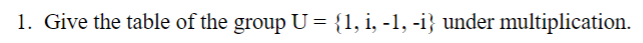
\includegraphics[]{sec4_extra1.PNG}
\newline
\begin{center}
    \setlength\doublerulesep{0pt}
    \begin{tabular}{r||*{4}{2|}}
    $\cdot$ & 1 & i & -1 & -i\\
    \hline\hline
    $1$ & 1 & i & -1 & -i\\
    \hline
    $i$ & i & -1 & -i & 1\\
    \hline
     $-1$ & -1 & -i & 1 & i\\
    \hline
    $-i$ & -i & 1 & i & -1\\
    \hline
    \end{tabular}
\end{center}

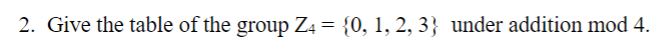
\includegraphics[]{sec4_extra2.PNG}
\newline

\begin{center}
    \setlength\doublerulesep{0pt}
    \begin{tabular}{r||*{4}{2|}}
        $+_4$ & $0$ & $1$ & $2$ & $3$\\
        \hline\hline
        $0$ & $0$ & $1$ & $2$ & $3$\\
        \hline
        $1$ & $1$ & $2$ & $3$ & $0$\\
        \hline
        $2$ & $2$ & $3$ & $0$ & 1\\
        \hline
        $3$ & $3$ & $0$ & $1$ & $2$\\
        \hline
    \end{tabular}
\end{center}

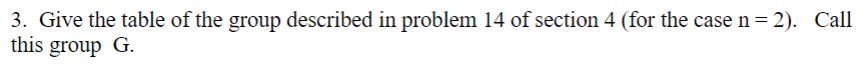
\includegraphics[]{sec4_extra3.PNG}
\newline


\begin{center}
    \setlength\doublerulesep{0pt}
    \begin{tabular}{c|| |c| |c| |c| |c| |c|}
    
        $\cdot$ &  $\begin{bmatrix*}[r]
            1 & 0\\
            0 & 1\\
        \end{bmatrix*}$ & $\begin{bmatrix*}[r]
            -1 & 0\\
            0 & 1\\
        \end{bmatrix*}$ & $\begin{bmatrix*}[r]
            1 & 0\\
            0 & -1\\
        \end{bmatrix*}$ & $\begin{bmatrix*}[r]
            -1 & 0\\
            0 & -1\\
        \end{bmatrix*}$\\
        \hline\hline
        
        $\begin{bmatrix*}[r]
            1 & 0\\
            0 & 1\\
        \end{bmatrix*}$ & $\begin{bmatrix*}[r]
            1 & 0\\
            0 & 1\\
        \end{bmatrix*}$ & $\begin{bmatrix*}[r]
            -1 & 0\\
            0 & 1\\
        \end{bmatrix*}$ & $\begin{bmatrix*}[r]
            1 & 0\\
            0 & -1\\
        \end{bmatrix*}$ & $\begin{bmatrix*}[r]
            -1 & 0\\
            0 & -1\\
        \end{bmatrix*}$\\
        \hline
        
        $\begin{bmatrix*}[r]
            -1 & 0\\
            0 & 1\\
        \end{bmatrix*}$ & $\begin{bmatrix*}[r]
            -1 & 0\\
            0 & 1\\
        \end{bmatrix*}$ & $\begin{bmatrix*}[r]
            1 & 0\\
            0 & 1\\
        \end{bmatrix*}$ & $\begin{bmatrix*}[r]
            -1 & 0\\
            0 & -1\\
        \end{bmatrix*}$ & $\begin{bmatrix*}[r]
            1 & 0\\
            0 & -1\\
        \end{bmatrix*}$\\
        \hline
        
        $\begin{bmatrix*}[r]
            1 & 0\\
            0 & -1\\
        \end{bmatrix*}$ & $\begin{bmatrix*}[r]
            1 & 0\\
            0 & -1\\
        \end{bmatrix*}$ & $\begin{bmatrix*}[r]
            -1 & 0\\
            0 & -1\\
        \end{bmatrix*}$ & $\begin{bmatrix*}[r]
            1 & 0\\
            0 & 1\\
        \end{bmatrix*}$ & $\begin{bmatrix*}[r]
            -1 & 0\\
            0 & 1\\
        \end{bmatrix*}$\\
        \hline
        
        $\begin{bmatrix*}
            -1 & 0\\
            0 & -1\\
        \end{bmatrix*}$ & $\begin{bmatrix*}[r]
            -1 & 0\\
            0 & -1\\
        \end{bmatrix*}$ & $\begin{bmatrix*}[r]
            1 & 0\\
            0 & -1\\
        \end{bmatrix*}$ & $\begin{bmatrix*}[r]
            -1 & 0\\
            0 & 1\\
        \end{bmatrix*}$ & $\begin{bmatrix*}[r]
            1 & 0\\
            0 & 1\\
        \end{bmatrix*}$\\
        \hline
    \end{tabular}
\end{center}

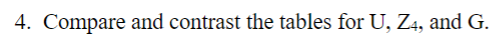
\includegraphics[]{sec4_extra4.PNG}
\newline

$U$ and $\mathbb{Z}_4$ have the form 
\begin{center}
    \setlength\doublerulesep{0pt}
    \begin{tabular}{r|| *{4}{2|}}
        $\cdot$ & e & a & b & c\\
        \hline\hline
        
        $e$ & e & a & b & c\\
        \hline
        
        $a$ & a & b & c & e\\
        \hline
        
        $b$ & b & c & e & a\\
        \hline
        
        $c$ & c & e & a & b\\
        \hline
    \end{tabular}
\end{center}

Where $e$ is the identity element for the group, and $a, b, c$ are members of the group. That is, $U$ and $\mathbb{Z}_4$ have the same structure, or are isomorphic. In contrast to $U$ and $\mathbb{Z}_4$, $G$ has the structure

\begin{center}
    \setlength\doublerulesep{0pt}
    \begin{tabular}{r||*{4}{2|}}
         $\cdot$ & e & a & b & c\\
         \hline\hline
         
         $e$ & e & a & b & c\\
         \hline
         
         $a$ & a & e & c & b\\
         \hline
         
         $b$ & b & c & e & a\\
         \hline
         
         $c$ & c & b & a & e\\
         \hline
    \end{tabular}
\end{center}

So $G$ is structurally different from $U$ and $\mathbb{Z}_4$. In other words, $G$ is not isomorphic to neither $U$ nor $\mathbb{Z}_4$.
\newline\newline


\Large{\textbf{Section 5 Problems}}
\newline

10. Determine if the set of upper-triangular $n \times n$ matrices with no zeros on the diagonal is a subgroup of $GL(n, \mathbb{R})$
\newline

Let $H$ be the set of all upper-triangular matrices with no zeros on the diagonal. Recall that the determinant of a triangular matrix is the product of the diagonal elements, and a matrix is invertible if and only if the determinant is non-zero. Since any element of $H$ has non-zero diagonal elements, its determinant will be non-zero. That is, any element of $H$ is an invertible $n \times n$ matrix. So $H$ is a subset of the set of all invertible matrices.
\newline

I claim that $\langle H, \cdot \rangle$ is a subgroup of $GL(n, \mathbb{R})$ where $\cdot$ is standard matrix multiplication.
\newline

Proof: We must first show that $H$ is closed under matrix multiplication. To begin, let $A, B \in H$ and consider $AB$. Recall that the $ij^{\text{th}}$ element of a matrix product is given by the following formula:

\begin{equation}
    ab_{ij} = \sum_{k = 1}^n a_{ik}b_{kj}
\end{equation}

where $ab_{ij}$ is the $ij^{\text{th}}$ element of $AB$ and $a_{ik}$ is the $ik^{\text{th}}$ element of $A$ and $b_{kj}$ is the $kj^{\text{th}}$ element of $B$. Since $A$ and $B$ are upper-triangular, the elements of $A$ and $B$ are strictly zero below the main diagonal. That is, $a_{ij} = b_{ij} = 0$ whenever $i < j$. Using equation (1), we will now show that the product of two upper-triangular matrices is also upper-triangular. In particular, we wish to show that $ab_{ij} = 0$ whenever $i < j$.
\newline

Well, whenever $i < j$, we have $a_{ij} = 0$ and $b_{ij} = 0$. Then from equation (1), for $k > i$, $a_{ik} = 0$. Similarly, for $k < j$, $b_{ij} = 0$. Now, since $i < j$, we cannot have $i = k = j$. That is to say, either $i < k$ or $k < j$. Then it will always be the case that $a_{ik} = 0$ or $b_{kj} = 0$. Then the sum in equation (1) must be equal to zero whenever $i < j$.
\newline

That is, for $i < j$, $ab_{ij} = 0$, so $AB$ is an upper-triangular matrix. So we have established that $H$ is closed under matrix multiplication. Now we must show that the identity element $e = I_n$ is in $H$.
\newline

Well, $I_n$ is a diagonal matrix, that is, zeros everywhere except the main diagonal. So, $I_n$ contains zeros in every element below the main diagonal, so $I_n \in H$. 
\newline

Now we must show that for any $A \in H$, $A^{-1} \in H$. That is, we must show that if $A$ is upper-triangular, $A^{-1}$ is also upper triangular. 
\newline

I will proceed by induction. We must first verify the base case ($n = 2$) holds. Recall that the inverse of a $2 \times 2$ matrix is given by the following:
\[
\begin{bmatrix}
    a & b\\
    c & d\\

\end{bmatrix}^{-1}
 = 
 \frac{1}{ad - cb}
 \begin{bmatrix}
    d & -b\\
    -c & a\\
 \end{bmatrix}
\]
Then for an upper triangular matrix, we have the following:
\[
\begin{bmatrix}
    a & b\\
    0 & c\\
\end{bmatrix}^{-1}
 = 
 \frac{1}{ac}
 \begin{bmatrix}
    c & -b\\
    0 & a\\
 \end{bmatrix}
\]
So we have that the inverse of a $2 \times 2$ upper-triangular matrix is also upper-triangular. Now assume this result holds to some natural number $n$. We must show that an $(n+1) \times (n+1)$ upper-triangular matrix's inverse is also upper-triangular. 
\newline

Well, by the induction hypothesis, the inverse of an $n \times n$ upper-triangular matrix is upper-triangular, so let $B$ be an $n \times n$ upper-triangular matrix of real entries and suppose without loss of generality that $B$ is not a diagonal matrix (the case where $B$ is diagonal is trivial since the inverse of a diagonal matrix is a diagonal matrix whose entries are the reciprocals of the original entries, both clearly upper-triangular) and let $B^{-1}$ be the inverse of B. 
\newline

Now let $B_1$ be an $(n+1) \times (n+1)$ upper-triangular matrix defined by the following:

\[B_1 = 
\begin{bmatrix}
    B & b_1\\
    \bm{0} & c\\
\end{bmatrix}\]
where $b_1 \in \mathbb{R}^n$ is a column vector, $\bm{0}$ is the $n$-dimensional row vector consisting only of zeros, and $c \in \mathbb{R}$. We wish to show that $B_1^{-1}$ is also upper-triangular. Suppose $B_1^{-1}$ can be written as the following:
\begin{equation}
B_1^{-1} = 
\begin{bmatrix}
    B^{-1} & b_{1}'\\
    b_{2}' & c'\\
\end{bmatrix}
\end{equation}
where $b_1' \in \mathbb{R}^n$ is a column vector, $b_2' \in \mathbb{R}^n$ is a row vector, and $c' \in \mathbb{R}$ is some number. We require that $B_1B_1^{-1} = B_1^{-1}B_1 = I_{n+1}$. Well,
\[B_1B_1^{-1} = 
\begin{bmatrix}
    B & b_1\\
    \bm{0} & c\\
\end{bmatrix}
\begin{bmatrix}
    B^{-1} & b_{1}'\\
    b_{2}' & c'\\
\end{bmatrix}
    =
\begin{bmatrix}
    BB^{-1} + b_1b_2' & Bb_1' + b_1c'\\
    cb_2' & cc'\\
\end{bmatrix}
\]
and
\[B_1^{-1}B_1 = 
\begin{bmatrix}
    B^{-1} & b_{1}'\\
    b_{2}' & c'\\
\end{bmatrix}
\begin{bmatrix}
    B & b_1\\
    \bm{0} & c\\
\end{bmatrix}
= 
\begin{bmatrix}
    B^{-1}B & B^{-1}b_1 + b_1'c\\
    b_2'B & b_2'b_1 + c'c\\
\end{bmatrix}
\]
Since the above two equations must be equal (and equal to $I_n$), we must have that $b_1b_2' = [0]_{n \times n}$ where $[0]_{n \times n}$ denotes the $n \times n$ matrix populated only by zeros, and $cb_2' = b_2'B$, and $cc' = 1$. 
\newline

From the equation $cb_2' = b_2'B$, we have $b_2' = b_2'(\frac{1}{c}B)$. For this to be true, it must be the case that either $B = cI_n$ or $b_2' = 0$. Well, since $B$ was assumed to not be a diagonal matrix, it cannot be the case that $B = cI_n$, so we have that $b_2' = 0$. Then from equation (2), we can see that $B^{-1}$ is upper triangular.
\newline

All of that work is to say that $\langle H, \cdot \rangle$ is indeed a group.
\newline\newline

12. Determine whether the set of $n \times n$ matrices with determinant $-1$ or $1$ is a subgroup of $GL(n, \mathbb{R})$.
\newline

Let $H$ be the set of all $n \times n$ matrices with determinant $-1$ or $1$. Notice that since any element of $H$ has non-zero determinant, $H \subseteq G$. I claim that $\langle H, \cdot \rangle$ is a subgroup of $GL(n, \mathbb{R})$ where $\cdot$ is the operation of matrix multiplication. 
\newline

Proof: We must first show that $H$ is closed under matrix multiplication. Let $M, N \in H$. Then $\text{det}(M) = \pm 1$ and $\text{det}(N) = \pm 1$. Consider the product $MN$ and find the determinant:
\[\text{det}(MN) = \text{det}(M)\text{det}(N) = (\pm 1) (\pm 1) = \pm 1\]
Then $MN \in H$, so $H$ is closed under matrix multiplication.

Now we must show the identity element $e = I_n \in H$. Well, $\text{det}(I_n) = 1$, so $I_n \in H$.

Finally, we must show for each $M \in H$, $M^{-1} \in H$ where $M^{-1}$ is the matrix inverse of $M$. Well, since $\text{det}(M) = \pm 1$, we have
\[\text{det}(M^{-1}) = \frac{1}{\text{det}(M)} = \frac{1}{\pm 1} = \pm 1\]
So $M^{-1} \in H$. 

That is, $\langle H, \cdot \rangle$ is a subgroup of $GL(n, \mathbb{R})$.
\newline\newline

For problems 15 and 16, let $F$ be the set of all real-valued functions with domain $\mathbb{R}$ and let $\tilde{F}$ be the subset of $F$ consisting of those functions that have a nonzero value at every point in $\mathbb{R}$. Determine whether the given subset of $F$ with the induced operation is (a) a subgroup of the group $F$ under addition, (b) a subgroup of the group $\tilde{F}$ under matrix multiplication.
\newline

15. The subset of all $f \in F$ such that $f(1) = 0$.
\newline

(a) Let $H = \{f \in F \: | \: f(1) = 0\}$. I claim that $\langle H, + \rangle$ is a subgroup of $\langle F, + \rangle$. 
\newline

Proof: We must begin by showing that $H$ is closed under addition. In particular, we must show that if $f, g \in H$, then $f + g \in H$. Well, since $f, g \in H$, we have $f(1) = 0$ and $g(1) = 0$. Then $(f + g)(1) = f(1) + g(1) = 0 + 0 = 0$, so $f + g \in H$. Then $H$ is closed under addition. 
\newline

Now we must show the identity element $e(x) = 0 \in H$. Well, notice $e(1) = 0$, so $e(x) \in H$. 
\newline

Finally, we must show that for any $f \in H$, its additive inverse $-f(x) \in H$. Well, for any $f \in H$, $f(1) = 0$, then $-f(1) = 0$, so $-f \in H$. So $\langle H, + \rangle$ is a subgroup of $\langle F, + \rangle$.
\newline

(b) Let $H$ be as in part (a) and $\cdot$ be multiplication. $\langle H, \cdot \rangle$ is NOT a subgroup of $\langle \tilde{F}, \cdot \rangle$ since for $f \in \tilde{F}$, $f(x) \neq 0$ for all $x \in \mathbb{R}$. That is to say, $H$ is not even a subset of $\tilde{F}$!
\newline


16. The subset of all $f \in \tilde{F}$ such that $f(1) = 1$.
\newline

(a) Let $H = \{f \in \tilde{F} \: | \: f(1) = 1\}$. $\langle H, + \rangle$ is not a subgroup of $\langle \tilde{F}, + \rangle$ since $H$ is not closed under addition! Let $f, g \in H$ and consider $f + g$. Notice that $(f + g)(1) = f(1) + g(1) = 1 + 1 = 2 \neq 1$, so $f + g \notin H$.
\newline

(b) Let $H$ be as in part (a). I claim that $\langle H, \cdot \rangle$ is a subgroup of $\langle \tilde{F}, \cdot \rangle$.
\newline

Proof: We must begin by showing that $H$ is closed under multiplication. Well, let $f, g \in H$ and consider $f \cdot g$. Notice that $f(1) \cdot g(1) = f(1)g(1) = (1)(1) = 1$. So $f \cdot g \in H$.
\newline

Now we must show that the identity element $e(x) = 1 \in H$. Well, notice $e(1) = 1$, so $e(x) \in H$. 
\newline

Finally, we must show for any $f \in H$, the inverse function $f^{-1} = \frac{1}{f} \in H$. Well, since $f \in H \subseteq \tilde{F}$, $f(x) \neq 0$ for all $x \in \mathbb{R}$ and so $\frac{1}{f}$ is defined for all $x \in \mathbb{R}$. Further notice that $\frac{1}{f(1)} = \frac{1}{1} = 1$ so $\frac{1}{f} \in H$. Thus we have established that $\langle H, \cdot \rangle$ is a subgroup of $\langle \tilde{F}, \cdot \rangle$.
\newline

34. Find the order of the cyclic subgroup of of the multiplicative group $G$ of invertible $4 \times 4$ matrices generated by
\[\begin{bmatrix}
    0 & 0 & 0 & 1\\
    0 & 0 & 1 & 0\\
    1 & 0 & 0 & 0\\
    0 & 1 & 0 & 0\\
\end{bmatrix}\]

Let $A$ be defined by the matrix above. We wish to find the set $\{A^n \: | \: n \in \mathbb{Z}\}$. Let us begin by calculating $A^2$:
\[A^2 = AA = 
\begin{bmatrix}
    0 & 0 & 0 & 1\\
    0 & 0 & 1 & 0\\
    1 & 0 & 0 & 0\\
    0 & 1 & 0 & 0\\
\end{bmatrix}
\begin{bmatrix}
    0 & 0 & 0 & 1\\
    0 & 0 & 1 & 0\\
    1 & 0 & 0 & 0\\
    0 & 1 & 0 & 0\\
\end{bmatrix}
=
\begin{bmatrix}
    0 & 1 & 0 & 0\\
    1 & 0 & 0 & 0\\
    0 & 0 & 0 & 1\\
    0 & 0 & 1 & 0\\
\end{bmatrix}
\]
Now $A^3$:
\[A^3 = A^2A = 
\begin{bmatrix}
    0 & 1 & 0 & 0\\
    1 & 0 & 0 & 0\\
    0 & 0 & 0 & 1\\
    0 & 0 & 1 & 0\\
\end{bmatrix}
\begin{bmatrix}
    0 & 0 & 0 & 1\\
    0 & 0 & 1 & 0\\
    1 & 0 & 0 & 0\\
    0 & 1 & 0 & 0\\
\end{bmatrix}
=
\begin{bmatrix}
    0 & 0 & 1 & 0\\
    0 & 0 & 0 & 1\\
    0 & 1 & 0 & 0\\
    1 & 0 & 0 & 0\\
\end{bmatrix}\]
And $A^4$:

\[A^4 = A^3A = 
\begin{bmatrix}
    0 & 0 & 1 & 0\\
    0 & 0 & 0 & 1\\
    0 & 1 & 0 & 0\\
    1 & 0 & 0 & 0\\
\end{bmatrix}
\begin{bmatrix}
    0 & 0 & 0 & 1\\
    0 & 0 & 1 & 0\\
    1 & 0 & 0 & 0\\
    0 & 1 & 0 & 0\\
\end{bmatrix}
=
\begin{bmatrix}
    1 & 0 & 0 & 0\\
    0 & 1 & 0 & 0\\
    0 & 0 & 1 & 0\\
    0 & 0 & 0 & 1\\
\end{bmatrix}\]

That is, every fourth power of $A$ will bring us to the identity matrix. Then we must have that this subgroup contains four elements, namely $I_4$, $A$, $A^2$, and $A^3$. That is, the order of this subgroup is four.
\newline

40. Show by means of example that it is possible for the quadratic equation $x^2 = e$ to have more than two solutions in some group $G$ with identity $e$.
\newline

Refer to problem 3 in the Section 4 Extra Problems. Notice that $G$ has four solutions to $x^2 = e$.
\newline

47. Prove that if $G$ is an abelian group, written multiplicatively, with identity element $e$, then all elements $x$ of $G$ satisfying the equation $x^2 = e$ form a subgroup $H$ of $G$.
\newline

Proof: Let $G$ be an abelian group, written multiplicatively with identity element $e$. Let $H = \{x \: | \: x \in G, \: x^2 = e\}$. We wish to show that $H$ is a subgroup of $G$. To begin, we must show that $H$ is closed under the operation on $G$. Let $x, y \in H$ and consider $x \cdot y$. We must show $(x \cdot y)^2 = e$.
\newline

Well,
\[(x \cdot y)^2 = (x \cdot y) \cdot (x \cdot y)\]
Since $G$ is abelian, we have $x \cdot y = y \cdot x$. Then the above equation becomes
\[(x \cdot y) \cdot (x \cdot y) = (x \cdot y) \cdot (y \cdot x)\]
By the associative property and the fact that $x^2 = e$ and $y^2 = e$, we have
\[ (x \cdot y) \cdot (y \cdot x)= x \cdot (y \cdot y) \cdot x = x\cdot y^2 \cdot x = x \cdot e \cdot x = x \cdot x = x^2 = e\]
So $xy \in H$.
\newline

Now we must show that the identity element $e \in H$. Well, notice $e^2 = e \cdot e = e$, so $e \in H$.
\newline

Finally, we must show that for any $x \in H$, the inverse element $x^{-1} \in H$. Since $G$ is a group, for any $x \in G$, $x$ has an identity element, call it $x^{-1}$, which is unique. Notice that since $x^2 = e$, $x^{-1} = x$, so $(x^{-1})^2 = e$. That is, $x^{-1} \in H$. 
\newline

So $H$ is a subgroup of $G$.


\end{document}
